% File: css-ot.tex

\documentclass{standalone}

\usepackage{tikz}
\usetikzlibrary{shapes, positioning, arrows.meta, calc, backgrounds, fit}

% default horizontal/vertical distance
\def\hdist{1.5}
\def\vdist{1.5}

\newcommand{\state}[3]{% #1: state name; #2: position; #3: state label
  \node (#1) [circle, inner sep = 0pt, minimum size = 10mm, text width = 10mm, align = center, draw, #2, font = \Large] {#3};
}

\newcommand{\trans}[5]{% #1: start state; #2: end state; #3: transition label; #4: transition label position; #5: style
  \draw[>=Stealth, ->,  #5] (#1) to node [rectangle, draw, above = 2pt, sloped, #4] {#3} (#2);
}

\newcommand{\transition}[4][]{% #2: start state; #3: end state; #4: transition label; #1: transition label position (optional)
  \draw[>=Stealth, ->] (#2) to node [rectangle, draw, above = 2pt, sloped, #1] {#4} (#3);
}

\tikzset{node distance = \vdist and \hdist}
\tikzset{path/.style = {draw, rounded corners, very thick, #1}}

\begin{document}
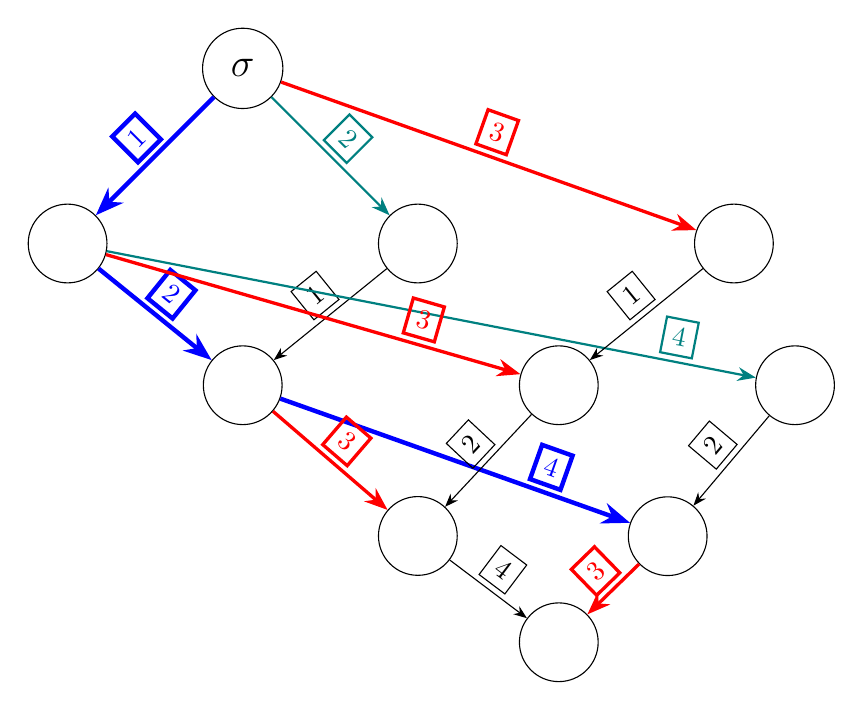
\begin{tikzpicture}
  \state{0}{}{$\sigma$}
  \state{1}{below left = of 0}{}
  \state{2}{below right = of 0}{}
  \state{12}{below = 2*\vdist of 0}{}
  \trans{0}{1}{1}{}{blue, ultra thick}
  \trans{0}{2}{2}{}{teal, thick}
  \trans{1}{12}{2}{}{blue, ultra thick}
  \trans{2}{12}{1}{}{}

  \state{3}{right = 2*\hdist of 2}{}
  \trans{0}{3}{3}{}{red, very thick}
  \state{14}{right = 4*\hdist of 12}{}
  \state{124}{below left = 0.80*\vdist and 0.6*\hdist of 14}

  \trans{1}{14}{4}{very near end}{teal, thick}
  \trans{12}{124}{4}{near end}{blue, ultra thick}
  \transition{14}{124}{2}

  \state{13}{right = 2*\hdist of 12}{}
  \trans{1}{13}{3}{near end}{red, very thick}
  \trans{3}{13}{1}{}{}

  \state{123}{below = 1.8*\vdist of 2}{}
  \trans{12}{123}{3}{}{red, very thick}
  \trans{13}{123}{2}{}{}

  \state{1234}{below = 1.5*\vdist of 13}{}
  \trans{123}{1234}{4}{}{}
  \trans{124}{1234}{3}{}{red, very thick}
\end{tikzpicture}
\end{document}
